% date: 2024-09-21
% Author: Bai Junhao
% Email: bjh2001@connect.hku.hk
% The University of Hong Kong

\documentclass{article}
\usepackage{fontspec}
\setmainfont{Times New Roman}

% Import necessary packages
\usepackage{amsmath}  % For mathematical expressions
\usepackage{amssymb}  % Additional math symbols
\usepackage{geometry}  % Set page geometry
\usepackage{graphicx}  % For adding images
\usepackage{fancyhdr}  % For custom headers and footers
\usepackage{titlesec}  % Control over title formatting
\usepackage{tocloft}   % Customizing table of contents
\usepackage{hyperref}  % For hyperlinks
\usepackage{ctex}      % For Chinese characters
\usepackage{color}     % For color in code listings
\usepackage{float}     % For floating figures
\usepackage{amssymb}   % For additional math symbols
\usepackage{listings}  % For code listings
\usepackage{enumitem}  % For customizing lists

% set equation numbering to section level
\numberwithin{equation}{section}

% set date language to en-US
\usepackage[english]{babel}

% Set page geometry
\geometry{a4paper, margin=1in}

% Set header and footer
\pagestyle{fancy}
\fancyhf{}  % Clear all header and footer fields
\fancyhead[L]{
\includegraphics[width=0.2\textwidth]{./img/HKU.png}}  % Add logo to the left of the header
\fancyhead[C]{\rightmark}  % Add current section title and number in the center of the header
\fancyfoot[C]{\thepage}  % Page number in the center of the footer

% Adjust headheight and topmargin
\setlength{\headheight}{25.27397pt}
\addtolength{\topmargin}{-4.3348pt}

% Ensure section marks are shown in the right format
\renewcommand{\sectionmark}[1]{\markright{\thesection\ #1}}

% Table caption and label formatting
\numberwithin{table}{section}
\numberwithin{figure}{section}


% Title setup
\title{
    \vspace{6cm}
    COMP 7503B - Multimedia technologies\\
    \vspace{0.5cm}
    \text{Assignment 1B}  % Subtitle text
    \vspace{1cm}
}
\author{Bai Junhao - 3036382909}  % Author
\date{\today}

% Reset page numbering after title page
\pagestyle{plain}
\begin{document}

% Title page
\maketitle
\thispagestyle{empty}  % No page number on title page

\newpage

% Table of Contents
\tableofcontents
% set page numbering to roman
\pagenumbering{roman}
\setcounter{page}{1}

\newpage

% Start page numbering from here
\pagenumbering{arabic}
\setcounter{page}{1}
% set page style to fancy
\pagestyle{fancy}

% Include the content from the file
% date: 2024-09-21
% Author: Bai Junhao
% Email: bjh2001@connect.hku.hk
% The University of Hong Kong

\section{Peter buttered the burnt toast}

\subsection{Question}
Launch the app on your mobile device in a quiet environment, speak the sentence “Peter buttered the burnt toast”. Take the screenshot of the spectrogram, and indicate the presence of the stop consonants and voiced phonemes in the spectrogram.

\subsection{Answer}
First we need to record this in a quiet environment. 
The Screenshot of the spectrogram is shown in Figure \ref{fig:Question1}.
\begin{figure}[H]
    \centering
    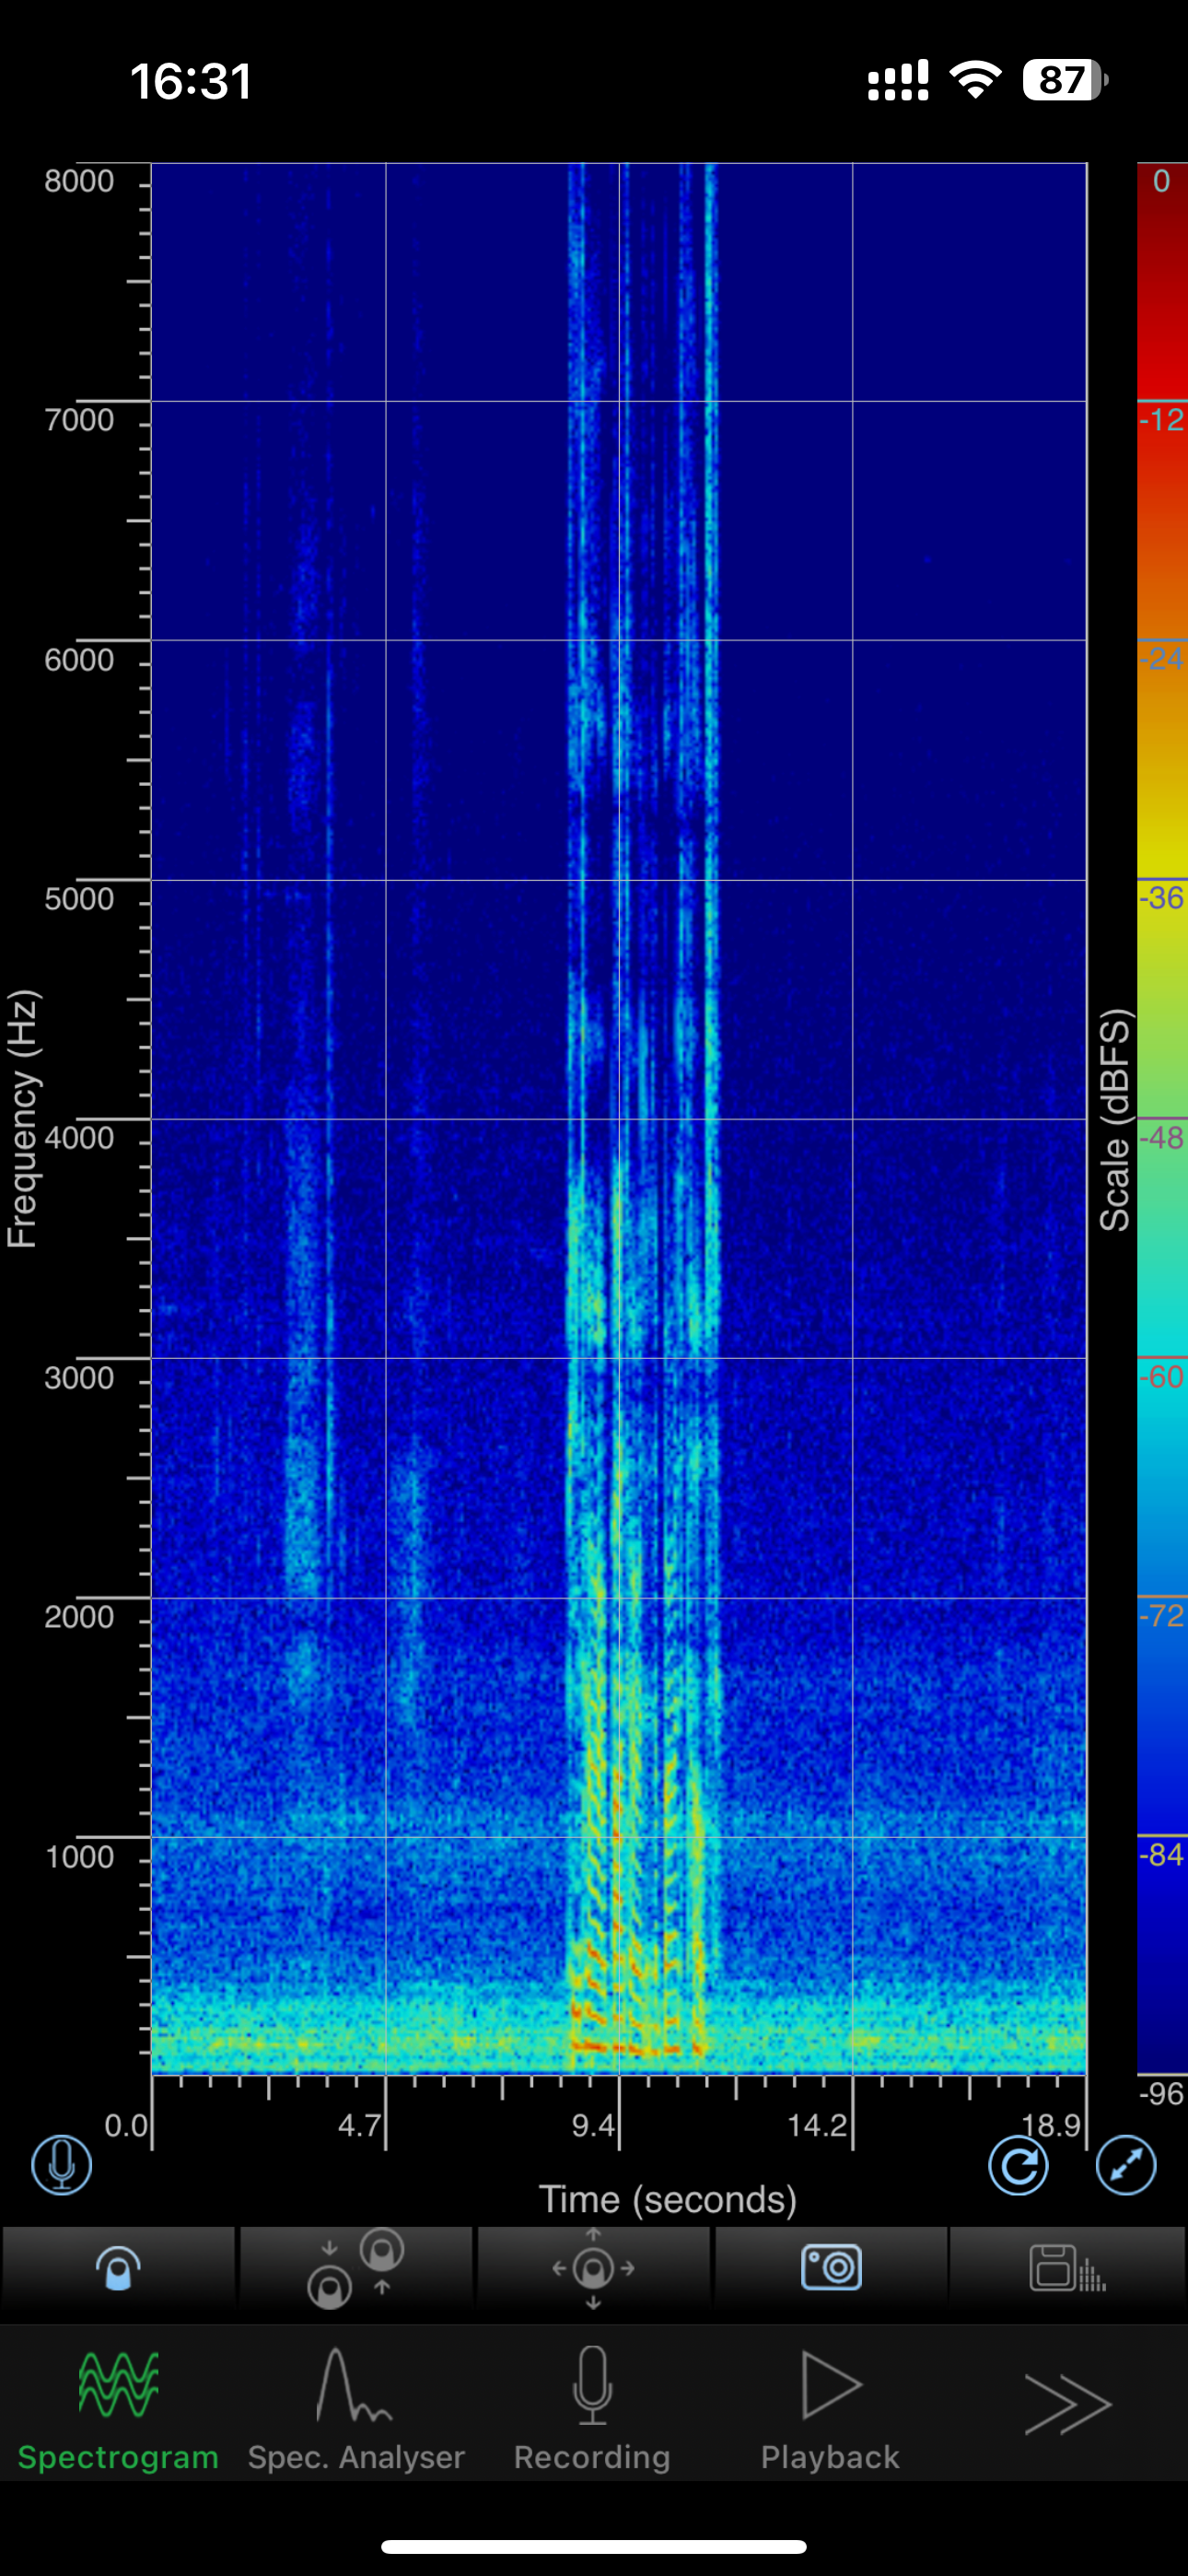
\includegraphics[width=0.4\textwidth]{./img/IMG_1831.PNG}
    \caption{Spectrogram of the sentence “Peter buttered the burnt toast”}
    \label{fig:Question1}
\end{figure}


Due to the inadequate scaling of the X-axis and Y-axis in the aforementioned figure, which does not effectively convey the desired experimental results, we have opted to utilize the recorded audio files and process them using relevant Python libraries.
The library used in this experiment is \texttt{librosa}. The code is shown in the following code block. The code reads the audio file, calculates the Short-Time Fourier Transform (STFT), and displays the spectrogram. The code also marks the voiced phonemes in the spectrogram.


\begin{figure}[H]
    \centering
    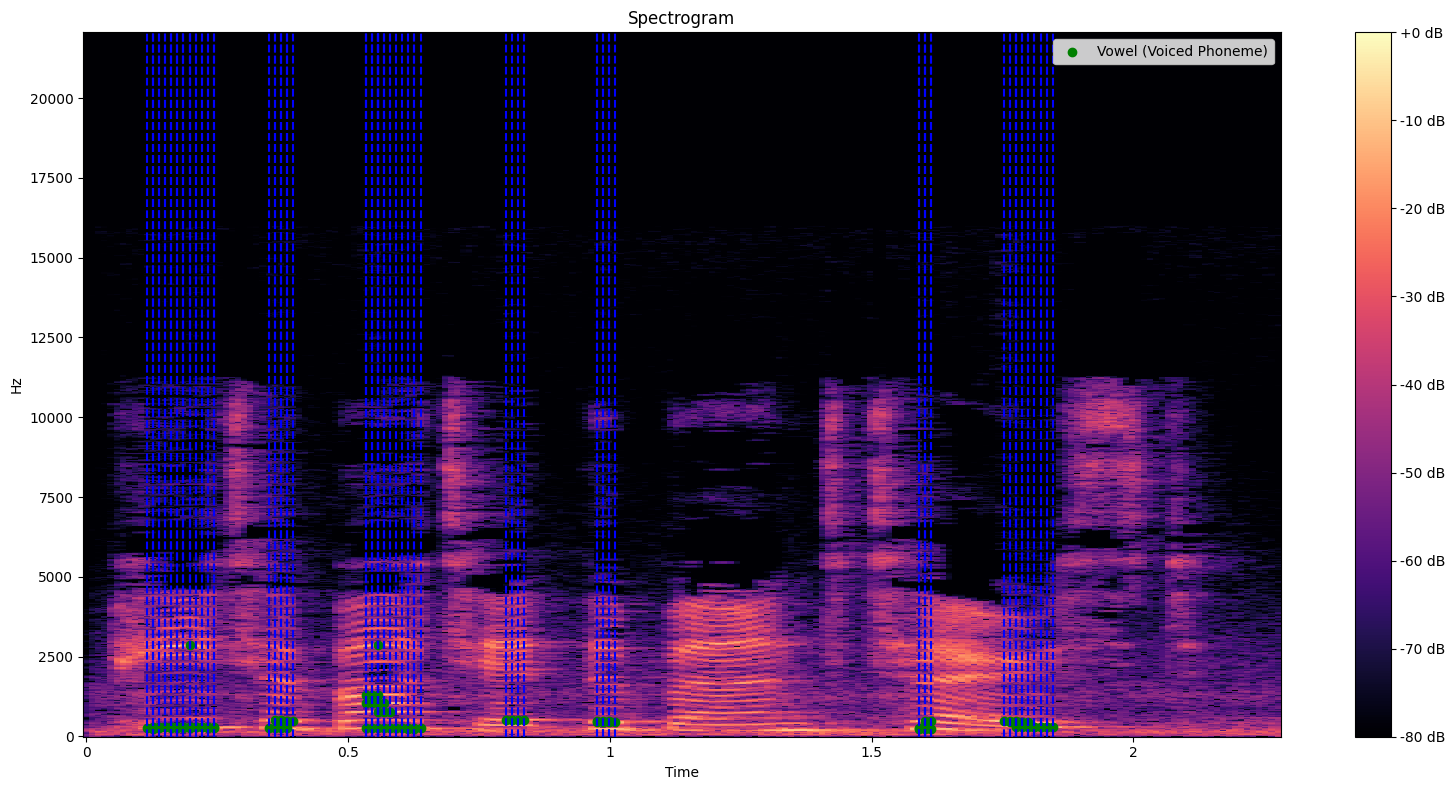
\includegraphics[width=\textwidth]{./img/Q1-1.png}
    \caption{Spectrogram of the sentence “Peter buttered the burnt toast”}
    \label{fig:Question1-2}
\end{figure}


From the figure \ref{fig:Question1-2}, the \textbf{green dots} and \textbf{blue line} indicate the sections corresponding to vowels (voiced phonemes). Additionally, there are several points where the frequency sharply rises; these points represent plosives, which are also known as stop consonants.

"Peter buttered the burnt toast" contains the following phonemes:

\begin{table}[H]
    \centering
    \begin{tabular}{|c|c|c|}
        \hline
        \textbf{Voiced Phonemes} & \textbf{Phonetic Representation} & \textbf{Count} \\ \hline
        Peter  & e, e & /i:/, /ə/ (2) \\ \hline
        buttered & u, ered & /ʌ/, /ɜ:/ (2) \\ \hline
        the & e & /ði:/ (1) \\ \hline
        burnt & u & /ɜ:/ (1) \\ \hline
        toast & oa & /əʊ/ (1) \\ \hline
        \textcolor{red}{\textbf{Total}} & & \textcolor{red}{7} \\ \hline
    \end{tabular}
    \caption{Phonemes in "Peter buttered the burnt toast"}
\end{table}

\vspace{1em} % Add some space between the tables
\begin{table}[H]
    \centering
    \begin{tabular}{|c|c|c|}
        \hline
        \textbf{Stop Consonants} & \textbf{Phonetic Representation} & \textbf{Count} \\ \hline
        Peter  & P, t & /p/, /t/ (2) \\ \hline
        buttered & b, t, d & /b/, /t/, /d/ (3) \\ \hline
        burnt & b, t & /b/, /t/ (2) \\ \hline
        toast & t, t & /t/, /t/ (2) \\ \hline
        \textcolor{red}{\textbf{Total}} & & \textcolor{red}{9} \\ \hline
    \end{tabular}
    \caption{Stop Consonants in "Peter buttered the burnt toast"}
\end{table}


/ð/ is a voiced dental fricative, representing the /th/ sound, as seen in the word "the." It does not belong to the categories of vowels or stop consonants; instead, it is classified as a fricative because the airflow creates friction between the tongue and the teeth during its production. In the spectrogram, there is a noticeable gap in the frequency domain.

Lastly, we can mark the voiced phonemes and stop consonants in the spectrogram. The updated spectrogram is shown in Figure \ref{fig:Question1-3}.

\begin{figure}[H]
    \centering
    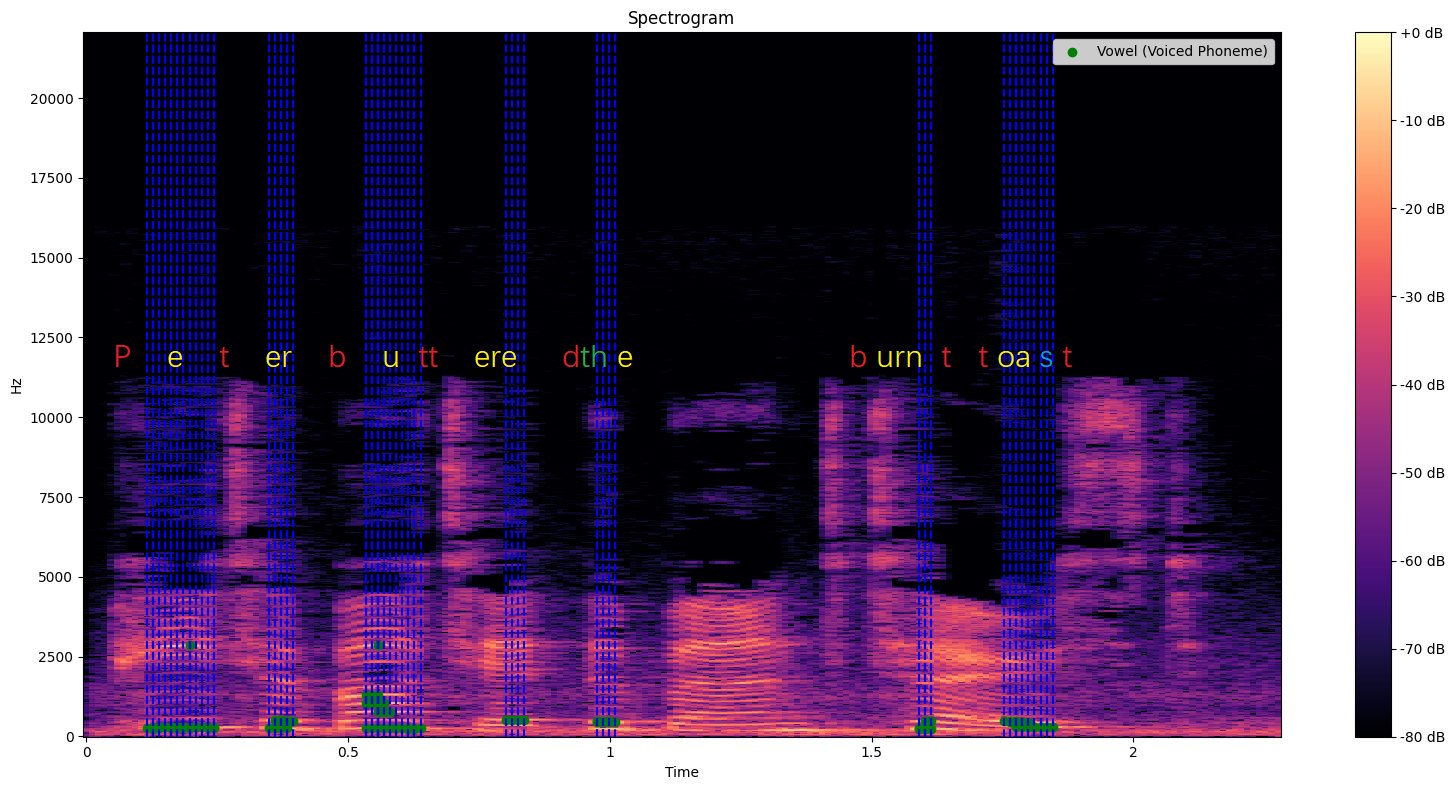
\includegraphics[width=\textwidth]{./img/Q1-2.png}
    \caption{Marked Spectrogram of the sentence “Peter buttered the burnt toast”}
    \label{fig:Question1-3}
\end{figure}

\subsection{Code}

\lstset{
    basicstyle=\small,
    breaklines=true,
    language=Python,
    showstringspaces=false,
    fontadjust=true
}
\begin{lstlisting}[language=Python, caption={Python code for Question 1}, label={code:Question1}, captionpos=b]
    import librosa
    import librosa.display
    import matplotlib.pyplot as plt
    import numpy as np

    # Read the audio file
    Q1, sr = librosa.load('./audio/Q1.wav', sr=44100)

    # Calculate the Short-Time Fourier Transform (STFT)
    D = librosa.amplitude_to_db(np.abs(librosa.stft(Q1)), ref=np.max)

    # Create a figure
    plt.figure(figsize=(16, 8))

    # Display the spectrogram
    librosa.display.specshow(D, sr=sr, x_axis='time', y_axis='linear')
    plt.colorbar(format='%+2.0f dB')
    plt.title('Spectrogram')

    # Define the frequency range for vowels
    vowel_freq_range = (200, 3000)
    threshold = -10

    # Get the frequencies
    freqs = librosa.fft_frequencies(sr=sr)
    vowel_indices = np.where((freqs >= vowel_freq_range[0]) & (freqs <= vowel_freq_range[1]))[0]

    # Find the high-energy indices
    high_energy_indices = np.where(D[vowel_indices, :] > threshold)

    # Convert the high-energy indices to time and frequency
    vowel_times = librosa.frames_to_time(high_energy_indices[1], sr=sr)
    vowel_freqs = freqs[vowel_indices[high_energy_indices[0]]]

    # Plot the voiced phonemes
    plt.scatter(vowel_times, vowel_freqs, color='g', marker='o', label='Vowel (Voiced Phoneme)')

    # Plot the stop consonants
    for time in vowel_times:
        plt.axvline(time, color='b', linestyle='--')

    # Add labels
    plt.legend(loc='upper right')

    # Display the plot
    plt.tight_layout()
    plt.show()
\end{lstlisting}

%
% End of Question 1

\newpage
% date: 2024-09-21
% Author: Bai Junhao
% Email: bjh2001@connect.hku.hk
% The University of Hong Kong

\section{I owe you a Yo-Yo}

\subsection{Question}
Repeat question 1 but this time with the sentence changed to ``I owe you a Yo-Yo''.

\subsection{Answer}
Similarly, following the approach of Question 1, we get the spectrogram of the sentence ``I owe you a Yo-Yo'' as shown in Figure \ref{fig:Question2}.

\begin{figure}[H]
    \centering
    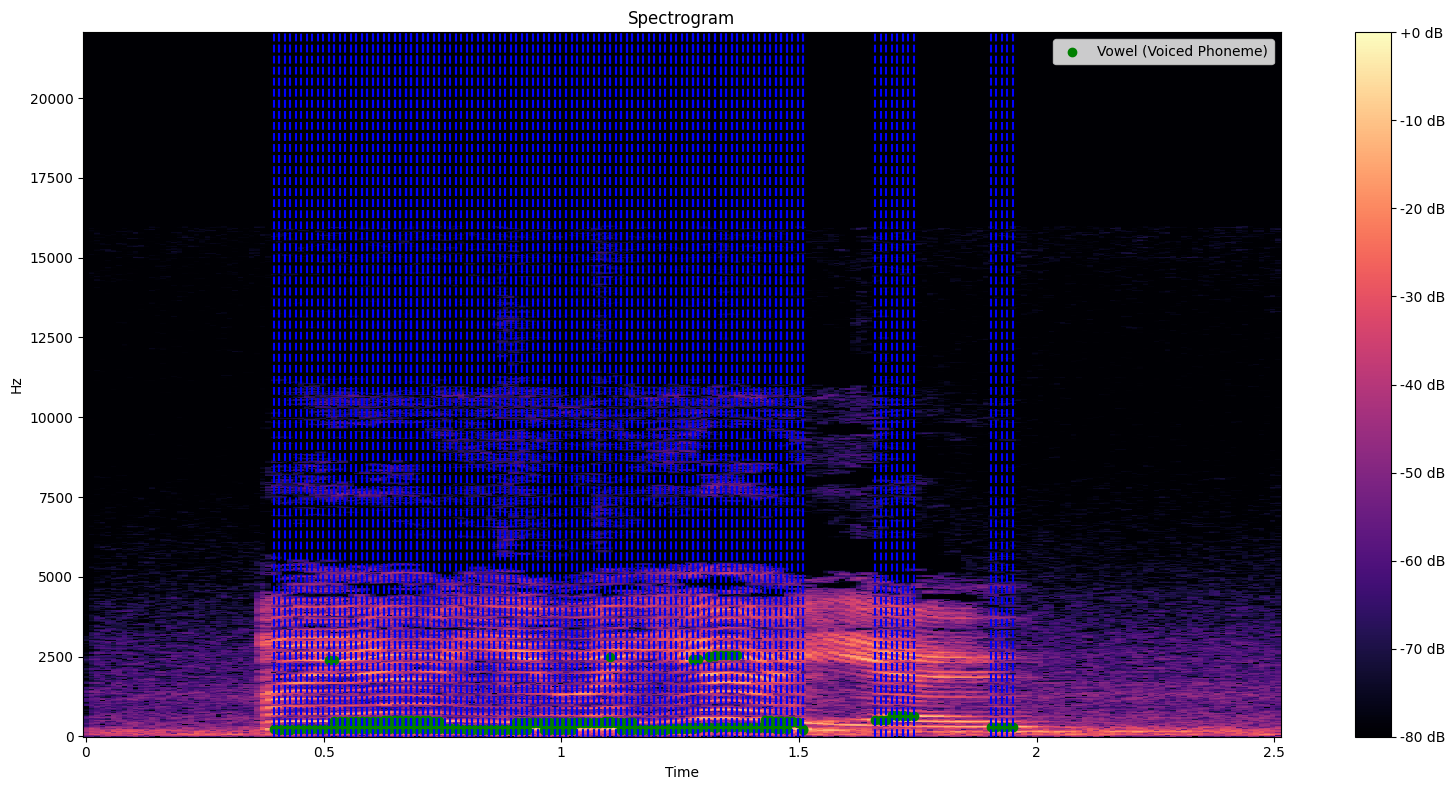
\includegraphics[width=\textwidth]{./img/Q2-1.png}
    \caption{Spectrogram of the sentence ``I owe you a Yo-Yo''}
    \label{fig:Question2}
\end{figure}

As observed in the spectrogram, the vowels in this sentence exhibit a higher concentration, which complicates the task of identifying the boundaries of the syllables. This overlapping of vowel sounds can create ambiguity, making it challenging for listeners to pinpoint where one syllable ends and another begins. However, a careful examination reveals that certain vowel sounds are notably continuous throughout the sentence. For instance, the vowel in ``I'' from the phrase ``I owe,'' the ``o'' in ``owe,'' the ``you'' in ``you a,'' and the ``a'' in ``a Yo-Yo'' all demonstrate a sustained presence.

In the spectrogram, these continuous vowel sounds are visually represented as straight lines, indicating their uninterrupted nature. This graphical representation suggests that these vowel sounds are held longer, contributing to the overall fluidity of the speech.

The number of vowels and consonants in this sentence are as follows:

\begin{table}[H]
    \centering
    \begin{tabular}{|c|c|c|}
        \hline
        \textbf{Voiced Phonemes} & \textbf{Phonetic Representation} & \textbf{Count} \\ \hline
        I  & I & /aɪ/ (1) \\ \hline
        owe & o, e & /əʊ/, /ʊ/ (2) \\ \hline
        you & u & /ju:/ (1) \\ \hline
        a & a & /eɪ/ (1) \\ \hline
        Yo-Yo & o, o & /əʊ/, /əʊ/ (2) \\ \hline
        \textcolor{red}{\textbf{Total}} & & \textcolor{red}{7} \\ \hline
    \end{tabular}
    \caption{Phonemes in ``I owe you a Yo-Yo''}
\end{table}

There's no stop consonants in this sentence, as all the consonants are fricatives or approximants.

\newpage
% date: 2024-09-21
% Author: Bai Junhao
% Email: bjh2001@connect.hku.hk
% The University of Hong Kong

\section{Obstacles in Word Segmentation}

\subsection{Question}

To implement speech to text algorithm, it is important to do word segmentation during spectrogram analysis. From what you observed in question 1 \& 2, explain why it is not easy to do word segmentation based on silence detection.

\subsection{Answer}

To implement a speech-to-text algorithm, word segmentation is a crucial step in the process of converting spoken language into written text. However, relying solely on silence detection to segment words, as observed from the spectrograms in Questions 1 and 2, presents several challenges.

Firstly, many sounds, particularly vowels, are continuous and lack clear pauses between them, even when moving from one word to another. For instance, in the sentence ``I owe you a Yo-Yo,'' the vowel sounds between words such as ``I'' and ``owe,'' or ``you'' and ``a,'' are continuous. In the spectrogram, these sounds often appear as uninterrupted bands, making it difficult to identify where one word ends and the next begins. This continuity of sound means that silence or significant pauses are not present between words, especially when the speech is fluid and natural, rather than deliberate.

Secondly, voiced phonemes (like vowels) often have higher energy levels and dominate the spectrogram, while unvoiced consonants or stop consonants (like ``p,'' ``t,'' ``b'') are brief and may not always be followed by noticeable silence. For example, in the phrase ``Peter buttered the burnt toast'' from Question 1, the stop consonants such as ``p'' and ``b'' are marked by short, sharp bursts of energy, but they are followed almost immediately by the vowels, leaving little to no silence for easy segmentation.

In natural speech, silence typically only occurs at the end of sentences or during intentional pauses, rather than between every word. This makes it unreliable to use silence as the primary method for word segmentation. Instead, more sophisticated techniques, such as detecting phoneme boundaries, stress patterns, or changes in frequency, are necessary for accurate segmentation in speech-to-text systems.

In summary, the absence of clear silences between words, the continuity of vowel sounds, and the brief nature of certain consonants make it difficult to rely on silence detection for word segmentation during spectrogram analysis.

\newpage
% date: 2024-09-21
% Author: Bai Junhao
% Email: bjh2001@connect.hku.hk
% The University of Hong Kong

\section{Importance of the Phonetic Alphabet in Voice Communication}

\subsection{Question}
Explain, by way of illustrating a number of sample spectrograms, why it is necessary to use phonetic alphabet (i..e A- Alpha, B - Beta, C - Charlie, …) to ensure correct exchange of letters over voice messages by radio or telephone.

\subsection{Answer}
The use of the phonetic alphabet (e.g., A for Alpha, B for Bravo, C for Charlie) is essential for ensuring the correct exchange of letters in voice communication, especially over radio or telephone, where audio quality may be compromised. This system provides clarity in distinguishing between letters that sound similar or may be misheard in noisy environments. By examining spectrograms, we can visually understand why this is necessary.

\subsubsection*{Similar Sounding Letters}
Certain letters in the English alphabet have phonemes that are acoustically similar, particularly under poor communication conditions. For instance, letters like "B" and "D" or "M" and "N" have similar stop consonants, and the difference between them may be subtle, especially in environments with background noise or signal interference. In a spectrogram, these letters may show similar patterns, with short bursts of energy followed by a vowel sound, making them hard to distinguish.

When the phonetic alphabet is used, however, these subtle differences become clearer. "B" is replaced by "Bravo," and "D" is replaced by "Delta," which not only introduces longer, distinct vowel sounds but also gives additional context. The spectrograms of "Bravo" and "Delta" show more distinguishable features with clear energy distribution over time, reducing confusion between the letters.

\subsubsection*{Dealing with Noisy Environments}
Radio and telephone communications often suffer from interference, distortion, or bandwidth limitations that can affect the clarity of speech. High-frequency noise or signal dropouts may mask critical parts of the speech signal, particularly affecting the stop consonants or fricatives in single-letter pronunciations like "F" and "S."

In spectrograms of real-world noisy communications, it's common to see sections of the signal interrupted by noise, particularly in the higher frequency ranges where consonants are more prominent. This can lead to misinterpretation of letters. Using a word from the phonetic alphabet like "Foxtrot" instead of "F" and "Sierra" instead of "S" provides more distinct visual and auditory cues, as these words have longer durations, clearer vowel transitions, and lower susceptibility to noise.

\subsubsection*{Clarity of Pronunciation}
Many letters in isolation are pronounced with very short sounds, which can lead to misinterpretation if the transmission quality is low. For instance, the letters "P," "T," and "K" are all short plosive sounds that may look similar on a spectrogram, as they have a rapid energy release followed by a brief period of silence. These letters, when transmitted over a low-quality connection, can be easily confused.

The phonetic alphabet elongates the transmission by incorporating longer, multi-syllabic words. The spectrograms of "Papa," "Tango," and "Kilo" show much more distinctive patterns, with clear vowel sounds separating the consonants. This helps prevent confusion by providing additional auditory information that is less likely to be lost in transmission.

\subsubsection*{Conclusion}
In summary, the use of the phonetic alphabet is crucial for ensuring the accurate exchange of letters over voice messages in challenging conditions. Spectrogram analysis highlights why this system is effective: it reduces ambiguity by replacing short, similar-sounding letters with longer, more distinct words that are easier to distinguish, even in noisy or degraded communication environments. The distinct visual representation of phonetic alphabet words on a spectrogram further demonstrates their clarity and robustness, making them indispensable for reliable voice communication.

\newpage

\end{document}
